\section{Il movimento open-source}

\subsection{Materiale di riferimento}

\begin{itemize}

\item \textit{The Daemon, the GNU and the Penguin: a history of Free and Open Source} - Peter Salus;\\
Capitoli 9, 18, 19, 20, 22 \\
Disponibile sotto Creative Common all'indirizzo: \url{http://www.debian.org/doc/manuals/project-history/}
\item \textit{Breve storia di Debian} - disponibile all'url: \url{http://www.debian.org/doc/manuals/project-history/}.
\item \textit{Lions' Commentary on UNIX 6th Edition, with Source Code} \url[http://v6.cuzuco.com/]

\end{itemize}

\subsection{MINIX}

Unix era un sistema operativo vero e proprio, ed era molto complesso. John Lions, un famoso sviluppatore Australiano, pubblica il codice sorgente commentato di UNIX in un'opera storica denominata: \textbf{Lions' Commentary on UNIX 6th Edition, with Source Code}. Ma con l'avvento della versione 7 di unix vengono imposti tutta una serie di blocchi: l'opera di Lyons viene bloccata, aumentano i costi delle licenze e vi sono delle restrizioni sull'insegnamento in classe. Molte università interruppero dunque l'insegnamento di unix; questo fu un cambiamento abbastanza stupido, perchè ciò che aveva reso forte unix era la diffusione nel mondo accademico. 

Andrew S. Tanenbaum era all'epoca un insegnante di \textit{computer science} e venne molto toccato da questa decisione, in quanto aveva sempre insegnato basandosi su unix. Decise allora di creare \textbf{MINIX}, un sistema operativo abbastanza importante, minimale, per scopi didattici, pensato per essere \textbf{semplice}. Era un sistema a micro kernel, rilasciato sotto \textbf{licenza permissiva} ma non libera. Aveva inoltre scritto un libro che documentava e spiegava MINIX. Ma questo sistema operativo aveva una grossa limitazione: \textbf{mancava un emulatore di terminale}.

\subsection{Linux}

Linus Torvalds è stato uno dei primi utilizzatori di MINIX. Nasce ad Helsinki nel 1969. Nel 1990 frequenta l'Università di Helsinki, comincia a studiare Tanenbaum e comincia a fare le prime modifiche per provare a creare un emulatore di terminale. Nel 1991 Lars Wirzenius (un amico di Torvalds) lo porta alla conferenza di Stallman, nella quale ebbe una prima esposizione al progetto GNU. Il 5 Gennaio 1991 Torvalds:

\begin{itemize}

\item Compra un PC (un 80386);
\item Ci installa MINIX;
\item Inizia a scriverci un emulatore di terminale (scritto in C e in assembly).

\end{itemize}

\begin{figure}[htbp]
\centering
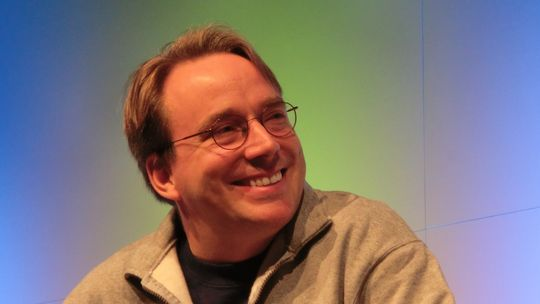
\includegraphics[width=50mm]{images/linus-torvalds.jpg}
\caption{Linus Torvalds}
\end{figure}

La prima versione di \textbf{Linux} è la A e la B, fatta solamente da due finestre. Da emulatore di terminale com'era pensato in origine Linux d lì il è stato espanso fino a crearci un vero e proprio sistema operativo \textbf{Linux 0.0.1} con un kernel funzionante.

Già nel 1992 il sistema era diventato molto importante. Torvalds decide dunque di rendere il sistema \textbf{indipendente} da MINIX (ci fu anche una disputa con Tanenbaum). Cambiò dunque la licenza adottando la GPL, che considerava buona per il suo sistema operativo, a prescindere dal software GNU stesso. Nascono inoltre già le prime distribuzioni basate su linux, come ad esempio SUSE, MCC o la prima distribuzione commerciale: LGX. Queste distribuzioni rendevano decisamente più facile l'utilizzo di Linux (di per sè molto complesso).

Nel 1994 viene rilasciato \textbf{Linux 1.0} e fu lo stesso Torvalds a presentarlo in una conferenza tenutasi ad Helsinki. Già allora era un sistema utilizzabile.

Ancora nel 1993 erano nate le prime versioni commerciali: Bolzern, Flagship e \textbf{Linux Pro}. Nel 1994 nasce inoltre \textbf{RedHat}, creato da Marc Ewing, e diventa ben presto la più diffusa distribuzione Linux.

Nel 1996 fu scelto come logo ufficiale di Linux un pinguino disegnato da Larry Ewing, chiamato \textbf{Tux}, come abbreviazione di \textbf{T}orvalds \textbf{U}nix.

Sempre nel 1996 esce \textbf{Linux 2.0} con supporto a microprocessore. Con la versione 3.0, uscita nel 2011, le modifiche sono state molto più incrementali. Nel corso degli anni con la 2.0 il grado di utenza era ancora molto piccolo.

\begin{table}[htpd]
\centering
	\begin{tabular}[c]{l | l | l}
	\hline
	& 1992 & 2012 \\
	\hline
	Sviluppatori Linux & 100 & 1000 \\
	\hline
	Linee di codice Linux & 250.000 & 14.000.000 \\
	\hline
	\end{tabular}
\caption{Sviluppo di Linux negli anni}
\end{table}

Una volta c'erano molti sviluppatori \textit{volontari}, ad oggi il supporto è dato da grosse aziende che possono investire tempo e denaro su Linux.

\subsection{Debian}

C'era un forte legame tra il mondo degli hackers e il mondo del software libero. Si venne a creare una \textbf{nuova generazione di sviluppatori}. Volevano provare a costruire una distribuzione che fosse fortemente legata a certi principi, che mettesse insieme varie cose, che facesse da collante. A quel punto nacque \textbf{Debian}. Linux da un lato stava procedendo e crescendo velocemente ed aveva molte caratteristiche interessanti, ma dall'altro c'era una lontananza dai principi del software libero e dalla GNU. Questo era percepito come un problema da parte di una fetta della comunità. Ad altri invece la cosa andava più che bene, dunque si venne a creare una \textbf{divergenza}. 

Il progetto Debian venne fondato da Ian Murdock nel 1993, con l'intento di fare una distribuzione di Linux \textbf{completamente libera}. Entrò a far parte del progetto GNU nel 1994-1995. Nel 1994 venne redatto il \textbf{manifesto debian}, nel quale si riassumeva il significato e la filosofia di debian. La prima versione stabile (Debian 1.1 ``Buzz'') venne rilasciata nel 1996. Il project leader della Debian divenne Bruce Perens

La caratteristica principale di Debian è che pone l'attenzione in modo quasi maniacale alla qualità del software (a volte perdendo anche molto tempo) e al fatto che il software sia libero (solo software DFSG. Si basa su una \textbf{forte comunità} che gestisce (tramite votazioni) tutte le decisioni sullo sviluppo; chiunque può proporre cambiamenti e ognuno è responsabile delle proprie azioni (attenzione alla sicurezza). Un altro cardine su cui puntano gli sviluppatori Debian è una strenua \textbf{disponibilità} del software.

Debian è caratterizzato da un suddivisione (politica) in più parti del repository. Le uniche componenti che sono della Debian sono quelle libere e quelle che dipendono da software libero. Il software che è all'interno della Debian entra nell'archivio principale, \textbf{FREE}. Poi all'interno ci sono altre componenti ospitate nel server della Debian ma che non sono della Debian, \textbf{NON-FREE} che non aderisce alle \textit{DFSG}, \textbf{CONTRIB} (che è libero ma dipende da componenti non libere).

C'è una versione di Debian \textbf{stabile} (software un po' vecchio però), quella che ha superato tutti i bugfix, una versione \textbf{non stabile} e una versione \textbf{testing}. Nella versione non stabile ``\textit{può esplodere tutto da un momento all'altro}'', viene aggiornata ogni giorno. La testing entra nel pacchetto solamente se nell'ultimo mese non sono stati segnalati bug importanti.

Da un lato Debian ha molto software e dall'altro non avendo interessi commerciali, non ha interessi nel penalizzare la concorrenza. È gestita essenzialmente da volontari.

\subsection{La cattedrale e il bazaar}

Un altro personaggio molto importante nel mondo del software libero è Eric Steven Raymond, informatico e programmatore statunitense di grande esperienza, che nel 1997 pubblica ``\textbf{La cattedrale e il bazaar}'', un saggio sullo sviluppo del software. Esso era essenzialmente destinato ad affrontare il problema del perchè Linux, con il suo kernel, funzionasse così bene. Non era scontato che Linux funzionasse, anzi all'inizio, secondo la sua opinione, era destinato a ``scoppiare''. Il problema è che ognuno tendeva a pensare con la propria testa; eppure la cosa non succedeva. Quindi iniziò ad analizzare il fenomeno. 

Una delle prime cose che ha fatto è stato quello di iniziare un progetto, chiamato \textbf{popclient}, per l'invio e la ricezione della posta. Comincia dunque ad utilizzare tutta una serie di principi per la gestione di questo progetto per vedere se riusciva a ricreare il successo che aveva visto con Linux, un progetto che funzionasse bene e avesse una solida base di sviluppatori. Uno dei principi che aveva adottato era di trattare gli utenti come una sorta di \textbf{co-sviluppatori}, come se il programma fosse stato fatto insieme a loro. La comunità popclient divenne dunque molto attiva. 

Il secondo principio su cui basò il proprio lavoro fu: ``Distribuisci presto, distribuisci spesso e presta ascolto agli utenti'', in questo modo si favorisce la risoluzione di bachi in tempi brevi. Molti utenti si facevano avanti e miglioravano il software, sentendosi parte attiva del progetto. L'idea che secondo Raymond aveva fatto il successo di Linux era trasformare il software da uno sviluppo di una persona che ``dona agli altri'' a uno sviluppo ``social'', attorno al quale ruotava una comunità. Spesso la varietà delle persone porta ad una varietà di modi per risolvere il problema, vi sono approcci diversi, e la combinazione dei contributi può significare grossi miglioramenti.

L'articolo di Raymond ebbe una grossissima fortuna, l'impatto all'interno della comunità fu molto sentito, e l'effetto di questo fu che l'attenzione andò oltre la semplice comunità degli appassionati. Una delle conseguenze di questo successo fu che nel 1998 Netscape annunciò di voler rilasciare il codice sorgente del proprio browser, e disse che per decidere questo si era basato anche sull'articolo di Raymond. Una volta Netscape era dominante, prima dell'arrivo del colosso Microsoft con Internet Explorer. Il browser di casa Microsoft è sicuramente disprezzato al giorno d'oggi, ma in realtà per gli standard di allora era molto buono e la Microsoft era riuscita, partendo da zero, a recuperare terreno in tempi notevoli su Netscape. A Netscape non interessava moltissimo del suo navigatore, non poteva infatti guadagnarci (era gratis), ma focalizzava la sua attenzione sul mondo Server. Temeva però che se Internet Explorer fosse divenuto dominante a quel punto i propri server sarebbero stati ``scartati'' in favore di quelli di Microsft. Avrebbe perso una grossa fetta di mercato e buona parte del loro reddito. Ebbero dunque l'idea di rilasciare il codice sorgente di Netscape sotto una licenza libera. In questa decisione aveva avuto un ruolo importante Raymond, che divenne dunque una celebrità.

C'era però il rischio che il termine ``software libero'' si svalutasse o non acquisisse la giusta importanza. Ci fu dunque una riunione su come sfruttare al massimo l'annuncio di Netscape: nasce il termine ``\textbf{open source}''. L'idea era che il software libero garantiva software di maggiore qualità ai fini di offrire una piattaforma stabile, con una buona comunità e aperta. Nel 1998 nasce dunque la \textbf{Open Source Initiative}, fondata da Raymodn e Perens, che aveva come scopo quello di diffondere il mondo open source. In questo movimento entrarono a far parte tutti gli sviluppatori più importante, come RedHat. 

\subsection{La filosofia open source}

Questi principi, che sono delle vere e proprie clausole, sono tutti pragmatici: quello che conta è costruire software che sia affidabile e veloce in modo analogo a Linux:

\begin{itemize}

\item \textbf{Licenze libere e permissive}; quando una licenza è chiusa si tratta gli utenti non come co-sviluppatori ma come ``utenti di serie B''. È come dire: ``\textit{Vabbè, se proprio vuoi fammi il bug reporting...}'' oppure ``\textit{Tu sei talmente inutile per me che nemmeno ti aiuto ad aiutarti...}''. È un principio che in casa Microsoft va bene, perchè l'obiettivo non è costruire una comunità. Nel caso del mondo open-source fare così è come ``darsi la mazza sui piedi'';
\item \textbf{Costruzione di una comunità attorno al software}; il software non è più una cosa che viene \textit{usata}, ma un modo di vivere, una cosa in cui le persone sono coinvolte. Con la crescita e lo sviluppo di una comunità attorno al software non solo i bachi vengono risolti più rapidamente, ma si hanno anche nuovi apporti mentali e contributi da parte delle persone;
\item \textbf{Trasparenza del processo di sviluppo}; la gente deve vedere quello che sta succedendo, perchè una volta che lo vede magari contribuisce. Questo tipo di comunicazione è fondamentale;
\item \textbf{Codice sorgente liberamente disponibile}; altrimenti non possono esserci trasparenza e contributi da parte della comunità;
\item \textbf{Codice sorgente liberamente modificabile};
\item \textbf{Libera redistribuzione}, anche ad uso commerciale;

\end{itemize}

\subsection{Open Source Definition}

L'Open Source Definition è nata perchè quando si è sviluppato il movimento OSI (\textit{Open Source Initiative}) ci si è reso conto che c'era il rischio, soprattutto nel momento in cui il movimento open source avesse avuto un forte impatto, che nella barca sarebbero saltati molti altri partecipanti ma non tutti avrebbero collaborato rispettando appieno le regole. Quindi era vitale decidere delle norme, delle linee guida da rispettare per scrivere del software open source. Esse erano pensate per escludere il minor numero di programmi già esistenti (esempio TEX, Perl, ...). Questo progetto ambiva a dare una caratterizzazione del software libero.

\subsubsection{Libera redistribuzione}

\begin{center}

\textit{La licenza non può limitare alcuno dal vendere o donare il software che ne è oggetto, come componente di una distribuzione aggregata, contenente programmi di varia origine. La licenza non può richiedere diritti o altri pagamenti a fronte di tali vendite.}

\end{center}

\textbf{Motivazione}: Imponendo la libera redistribuzione, si elimina la tentazione di rinunciare a importanti guadagni a lungo termine in cambio di un guadagno materiale a breve termine, ottenuto con il controllo delle vendite. Se non vi fosse questa imposizione, i collaboratori esterni sarebbero tentati di abbandonare il progetto, invece che di farlo crescere.

\subsubsection{Codice sorgente}

\begin{center}

\textit{Il programma deve includere il codice sorgente e ne deve essere permessa la distribuzione sia come codice sorgente che in forma compilata. Il codice sorgente deve essere il formato preferito per effettuare modifiche al codice.}

\end{center}

\textbf{Motivazione}: si richiede l'accesso al codice sorgente poichè non si può far evolvere un programma senza poterlo modificare. Il nostro obiettivo è rendere facile l'evoluzione del software, pertanto richiediamo che ne sia resa facile la modifica.

\subsubsection{Prodotti derivati}

\begin{center}

\textit{La licenza deve permettere modifiche e prodotti derivati, e deve permetterne la redistribuzione sotto le stesse condizioni della licenza del software originale.}

\end{center}

\textbf{Motivazione}: la sola possibilità di leggere il codice sorgente non è sufficiente a permettere la revisione indipendente del software da parte di terzi e una rapida selezione evolutiva. Per garantire una rapida evoluzione, deve essere possibile sperimentare modifiche al software e redistribuirle.

\subsubsection{Discriminazione contro persone o gruppi}

\begin{center}

\textit{La licenza non deve discriminare alcuna persona o gruppo di persone.}

\end{center}

\textbf{Motivazione}: per ottenere il massimo beneficio dal processo, il massimo numero di persone e gruppi deve avere eguale possibilità di contribuire allo sviluppo del software. Pertanto viene proibita l'esclusione arbitraria dal processo di persone o gruppi.

\subsubsection{Integrità del codice sorgente originale}

\begin{center}

\textit{La licenza può impedire la distribuzione del codice sorgente in forma modificata, a patto che venga consentita la distribuzione dell'originale accompagnato da ``patch'', ovvero file che permettono di applicare modifiche al codice sorgente in fase di compilazione.}

\end{center}

\textbf{Motivazione}: incoraggiare il miglioramento è bene, ma gli utenti hanno diritto di sapere chi è responsabile del software che stanno usando. Gli autori e i tecnici hanno diritto reciproco di sapere cosa è loro chiesto di supportare e di proteggersi la reputazione.

\subsubsection{Discriminazione per campo d'applicazione}

\begin{center}

\textit{La licenza non deve impedire di far uso del programma in un ambito specifico.}

\end{center}

\textbf{Motivazione}: L'intenzione principale di questa clausola è di proibire trappole nelle licenze che impediscano al software open source di essere usato commercialmente. Vogliamo che le aziende si uniscano alla nostra comunità, non che se ne sentano escluse.

\subsubsection{Distribuzione della licenza}

\begin{center}

\textit{I diritti allegati a un programma devono essere applicabili a tutti coloro a cui il programma è redistribuito, senza che sia necessaria l'emissione di ulteriori licenze.}

\end{center}

\textbf{Motivazione}: questa clausola intende proibire la chiusura del software per mezzi indiretti, come un obbligo di sottoscrizione di accordi di non diffusione.

\subsubsection{Specificità ad un prodotto}

\begin{center}

\textit{I diritti allegati al programma non devono dipendere dall'essere il programma parte di una particolare distribuzione del software.}

\end{center}

\textbf{Motivazione}: questa clausola impedisce un'ulteriore classe di licenze-trappola

\subsubsection{Vincoli su altro software}

\begin{center}

\textit{La licenza non deve porre restrizioni su altro software distribuito insieme al software licenziato.}

\end{center}

\textbf{Motivazione}: i distributori di software open source hanno il diritto di fare le loro scelte riguardo al software che intendono distribuire.

\subsubsection{Neutralità rispetto alle tecnologie}

\begin{center}

\textit{La licenza non deve contenere clausole che dipendano o si basano su particolari tecnologie o tipi di interfacce.}

\end{center}

\textit{Nota}: no al mouse click obbligatorio.

\subsection{Libertà del software libero}

\begin{itemize}

\item Libertà di eseguire il programma per qualsiasi scopo;
\item Libertà di studiare il programma e modificarlo;
\item Libertà di redistribuire copie del programma in modo da aiutare il prossimo;
\item Libertà di migliorare il programma e di distribuire pubblicamente i miglioramenti, in modo tale che tutta la comunità ne tragga beneficio.

\end{itemize}